\documentclass{standalone}
\usepackage{tikz}
\usetikzlibrary{arrows,positioning} 
\usetikzlibrary{fit}
\usetikzlibrary{shadows}

\tikzset{
	%Define standard arrow tip
	>=stealth',
	%Define style for boxes
	punkt/.style={
		rectangle,
		rounded corners,
		draw=black, very thick,
		text width=4.5em,
		minimum height=1.5em,
		text centered},
	% Define arrow style
	pil/.style={
		->,
		thick,
		shorten <=2pt,
		shorten >=2pt,}
}

\begin{document}
	
	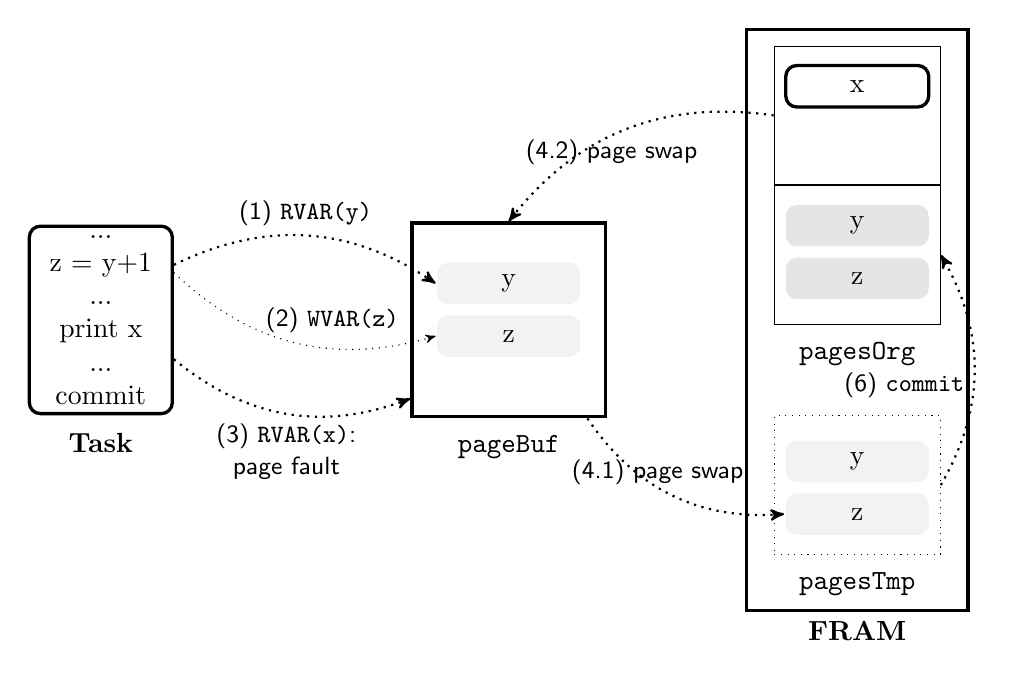
\begin{tikzpicture}[node distance=1cm, auto,]
	
	\node[punkt,minimum height=3em] (task1) {...\\z = y+1 \\ ... \\ print x \\ ... \\ commit};
	\node[below = 0.1cm of task1] () {\textbf{Task}};
	
	\node[draw,very thick,minimum width=7em, minimum height=7em, right = 3cm of task1] (sram) {};
	\node[below = 0.1cm of sram] () {\texttt{pageBuf}};
	
	\node[punkt,draw=none, below = -2cm of sram,fill=black!5] (y-sram) {y};
	\node[punkt,draw=none, below = 0.1cm of y-sram,fill=black!5] (z-sram) {z};
	
	\node[right = 0.5cm of sram] (ref) {};
	\node[draw,very thick,minimum width=8em, minimum height=21em, right = of ref] (fram1) {};
	
	\node[draw,above = -2cm of fram1,minimum width=6em, minimum height=5em] (pagesOrg1) {};
	\node[draw,below = 0 cm of pagesOrg1,minimum width=6em, minimum height=5em] (pagesOrg2) {};
	\node[below = 0.1cm of pagesOrg2] (original) {\texttt{pagesOrg}};
	
	\node[punkt, above = -0.8cm of pagesOrg1] (x1-fram) {x};
	\node[punkt,draw=none, above =-0.8cm of pagesOrg2,fill=black!10] (y1-fram) {y};	
	
	\node[punkt,draw=none, below = 0.1cm of y1-fram,fill=black!10] (z1-fram) {z};
	
	\node[draw,dotted,below = -2.5cm of fram1,minimum width=6em, minimum height=5em] (pagesTmp) {};
	\node[punkt,draw=none, below = -2.2cm of fram1,fill=black!5] (y2-fram) {y};
	\node[punkt,draw=none, below = 0.1cm of y2-fram,fill=black!5] (z2-fram) {z};
	
	\node[below = 0.1cm of pagesTmp] (copies) {\texttt{pagesTmp}};	
	
	\node[below = 0cm of fram1] () {\textbf{FRAM}};
	
	\path[every node/.style={font=\sffamily\small}]
	([yshift=0.6cm] task1.east) edge [->, bend right,dotted] node[xshift=-0.5cm]  {(2) \texttt{WVAR(z)} } (z-sram.west)
	
	([yshift=0.7cm]task1.east) edge [->, bend left,dotted,thick] node[xshift=-1cm] {(1) \texttt{RVAR(y)}} (y-sram.west)
	
	([yshift=-0.5cm]task1.east) edge [->, bend right,dotted,thick] node[below] { \shortstack{(3) \texttt{RVAR(x)}:\\ page fault}} ([yshift=-1cm]sram.west)
	
	([xshift=1cm]sram.south) edge [->, bend right,dotted,thick] node[xshift=-1.4cm] {(4.1) page swap} (z2-fram.west)
	
	(pagesOrg1.west) edge [->, bend right,dotted,thick] node[xshift=-1.4cm] {(4.2) page swap} (sram.north)
	
	(pagesTmp.east) edge [->, bend right,dotted,thick] node[yshift=-0.2cm]{(6) \texttt{commit}} (pagesOrg2.east);
	
	\end{tikzpicture}
	
\end{document}